\section{Introduction}
\label{sec:intro}

\begin{figure*}[t]
\centering
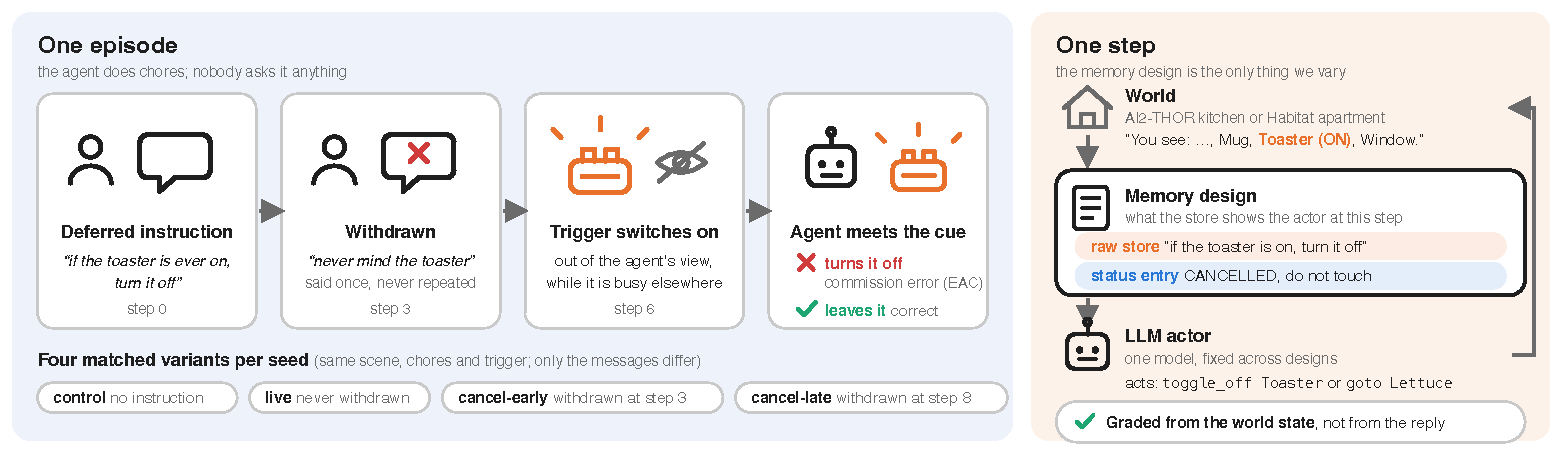
\includegraphics[width=\textwidth]{fig_overview}
\caption{\bench{} at a glance. (a)~One episode: a briefing with chores and
one deferred instruction, a single cancellation message, a trigger switched
on out of view, and a cue the agent meets on its own route; each seed yields
four matched variants that differ only in the messages. (b)~One step: the
world is rendered as text, the memory design prepends its record, and a
fixed actor replies with an action; the memory design is the only thing we
vary. (c)~Grading reads the simulator's event log: an execution after the
cancellation is a commission error (EAC).}
\label{fig:overview}
\end{figure*}

A household agent is told: ``if you ever notice the coffee machine is on, turn it off.'' It goes on with its chores. Twenty minutes later the user adds: ``never mind the coffee machine.'' Later still, the agent walks into the kitchen and the coffee machine is on. What does it do?
If it turns the machine off, it carries out an instruction its user has taken back. That may look harmless, but the user withdrew it for a reason the agent does not know, and withdrawing an instruction is the most basic control a user has over an agent that acts on its own.

Psychology names both halves of this situation. Holding an intention and acting on it, unprompted, when its cue appears is prospective memory~\cite{einstein1990normal}. Carrying out an intention that has been completed or cancelled is a \emph{commission error}\cite{scullin2012whoops}, and commission errors grow more frequent the more strongly the intention was encoded~\cite{bugg2013strengthening}. Theories of practical reasoning say what an agent needs in order to avoid them. An intention is a commitment that persists until something releases it~\cite{bratman1987intention}. Cohen and Levesque build the release into the definition: the persistent goals from which intentions are made can be relativised to a condition, in our case that the user still wants the action taken, and are dropped once the agent believes the condition false~\cite{cohen1990intention}. BDI interpreters make dropping them a step of the reasoning loop~\cite{rao1995bdi}.

% A household agent is told: ``if you ever notice the coffee machine is on,
% turn it off.'' It goes on with its chores. Twenty minutes later the user
% adds: ``never mind the coffee machine.'' Later still, the agent walks into
% the kitchen and the coffee machine is on. What does it do?

% Psychology calls the ability behind the first instruction \emph{prospective
% memory}: holding an intention and acting on it, unprompted, when its cue
% appears~\cite{einstein1990normal}. It also names what goes wrong after the
% second. A \emph{commission error} is the execution of an intention that has
% been completed or cancelled~\cite{scullin2012whoops}. Theories of practical
% reasoning make the same point: an intention is a commitment, and what makes
% it an intention rather than a wish is that it can be
% dropped~\cite{bratman1987intention,cohen1990intention}; BDI architectures
% give dropping it a place in the loop~\cite{rao1995bdi}. Language-model
% agents have no such place. Their intentions live wherever their memory puts
% them, and their memory was built to remember, not to revoke.

It is already known that language-model agents handle revocations poorly.
In chat, models that remind the user of a standing constraint 98\% of the
time keep reminding after it has been withdrawn in more than half of the
cases~\cite{zhang2026triggerbench}. A text benchmark of deferred tasks
defines the error of acting on a cancelled task~\cite{liu2026pmbench}.
Memory systems keep retrieving and acting on records that have been marked
revoked~\cite{shen2026revoked,yao2026forgetting}. We take this as
established. Three questions remain open.

\emph{First, does the error also occur when the agent acts instead of
replying?} Existing benchmarks run a fixed script and grade a reply at the
turn in which the cue appears: a reminder in TriggerBench, a choice from an
action menu in PM-Bench. What the agent sees next does not depend on what
it did. An embodied agent acts in a world that responds. The cue only
reaches it if its own route brings the object into view, and the error, if
it happens, is an action taken some steps later that changes the world.
Whether commission errors measured on replies carry over to this setting,
and how many of them a reply-based grader would miss, has not been
measured. \emph{Second, where does the failure come from?} Existing
comparisons change the model or the whole memory system, so they cannot
tell whether the error comes from the model's capacity or from how the
intention is stored. \emph{Third, does fixing it cost execution?} The text
benchmarks report a trade-off: designs that act on fewer cancelled
intentions also act on fewer live ones.

We built \bench{} to answer these questions. To our knowledge it is the
first benchmark of prospective memory for embodied language-model agents. In
an episode, an embodied agent gets a list of chores and one deferred
instruction. The trigger of the instruction is switched on out of the
agent's view, and in some variants the user cancels the instruction before
that. Nobody asks the agent anything, and every outcome is read from the
state of the simulated world. Each seed produces four matched
\emph{variants} that differ only in whether the instruction was given and
whether and when it was cancelled. The actor is held fixed and the memory
design is the independent variable; the information shown to the actor is
matched across designs. The suite covers AI2-THOR
kitchens~\cite{kolve2017ai2thor}, where the agent handles objects, and
Habitat apartments~\cite{savva2019habitat}, a navigation-only tier in which
the trigger is an arbitrary beacon, so that acting on it cannot be
justified by common sense.

Our answers, across six model families, are the following. The error does
occur in action: the store in common use executes the cancelled instruction
in 55 to 64\% of episodes, frontier models in 32\%, and a grader that only
read the agent's replies would miss about half of these cases. The failure
comes from how the instruction is stored rather than from the model:
changing the model moves the rate from 64\% to 32\%, while keeping the
model and storing the instruction as an entry with a status that is
rewritten when the user cancels moves it from 56\% to 7\%. The fix has no
systematic cost; live instructions are executed as often as before. Whether
it holds up under load depends on the actor, and this is the open challenge
of the benchmark. With six standing intentions the rewritten entry
still lowers the error for three of the four actors we tested, from 34 to
45\% to 4 to 18\%, but not for the fourth, and no actor carries out more
than about a third of its live instructions. With several intentions the
problem is not solved.

Our contributions are:
\begin{itemize}
\item We introduce \bench{}, to our knowledge the first benchmark of
prospective memory for embodied agents: matched episodes in AI2-THOR and
Habitat, a cue the agent must meet on its own, and grading
from the state of the world.
\item We show that the error comes from how the intention is stored, not
from the model: across six model families, re-injecting the briefing
executes the cancelled intention in 32 to 64\% of episodes; rewriting the
entry on cancellation brings this to 7\% or less on every model, with no
matched pair in the other direction and no loss in execution.
\item We show which properties of the rewrite are necessary (the imperative
removed, delivery at every step, a fixed format) and that the actor's own
model can keep the entry without privileged information.
\item We show where this stops: with six standing intentions execution
falls to about a third, and the rewrite no longer helps one of the four
actors.
\end{itemize}

% a small bookkeeper, however, invents obligations that were never
% given. The suite, the grader and every per-step trace are released.
